\documentclass[border=3pt]{standalone}
% Preâmbulo compartilhado pelos diagramas TikZ da aula 10 (Localização de Markov e Gaussiana)
\usepackage[T1]{fontenc}
\usepackage[utf8]{inputenc}
\usepackage{lmodern}
\usepackage{amsmath}
\usepackage{xcolor}
\usepackage{tikz}
\usetikzlibrary{arrows.meta,angles,quotes,decorations.pathmorphing,calc,
                positioning,shapes.geometric,shapes.misc,backgrounds,fit,
                math}

% Paleta (mesma dos SVGs originais)
\definecolor{dblue}{HTML}{2A5B8C}
\definecolor{dorange}{HTML}{B3541E}
\definecolor{dgreen}{HTML}{4A7C59}
\definecolor{dred}{HTML}{9C4B4B}
\definecolor{dcream}{HTML}{F4F1EA}
\definecolor{dshade}{HTML}{DDD7C9}

% Função gaussiana (não normalizada por padrão de escala visual)
\pgfmathdeclarefunction{gauss}{3}{%
  \pgfmathparse{1/(#3*sqrt(2*pi))*exp(-((#1-#2)^2)/(2*#3^2))}%
}

% Estilos comuns (prefixo d... para não colidir com chaves internas do pgf)
\tikzset{
  >={Stealth[length=2mm]},
  dguide/.style={gray!55, dashed, line width=0.4pt},
  daxis/.style={gray!60, line width=0.7pt, ->},
  dbody/.style={fill=black!3, draw=black!80, line width=1pt},
  dacc/.style={draw=dblue, line width=1pt},
  dlbl/.style={black!55, font=\small},
  dsub/.style={black!45, font=\footnotesize},
  dstate/.style={circle, draw=black!80, fill=dcream, line width=1pt,
                 minimum size=17mm, font=\large, inner sep=1pt},
  dobs/.style={circle, draw=black!80, fill=dshade, line width=1pt,
               minimum size=14mm, font=\large, inner sep=1pt},
  dbox/.style={rounded corners=2pt, draw=black!80, fill=dcream, line width=1pt,
               align=center, inner sep=6pt},
  dop/.style={circle, draw=black!80, fill=white, line width=1pt,
              minimum size=6mm, inner sep=0pt, font=\small},
  dtrans/.style={->, dblue, line width=1pt},
  dmeas/.style={->, dorange, line width=1pt},
  dcurve/.style={line width=1pt, dblue},
  dcurveb/.style={line width=1.4pt, dorange},
}

\usetikzlibrary{shapes.callouts}
\begin{document}
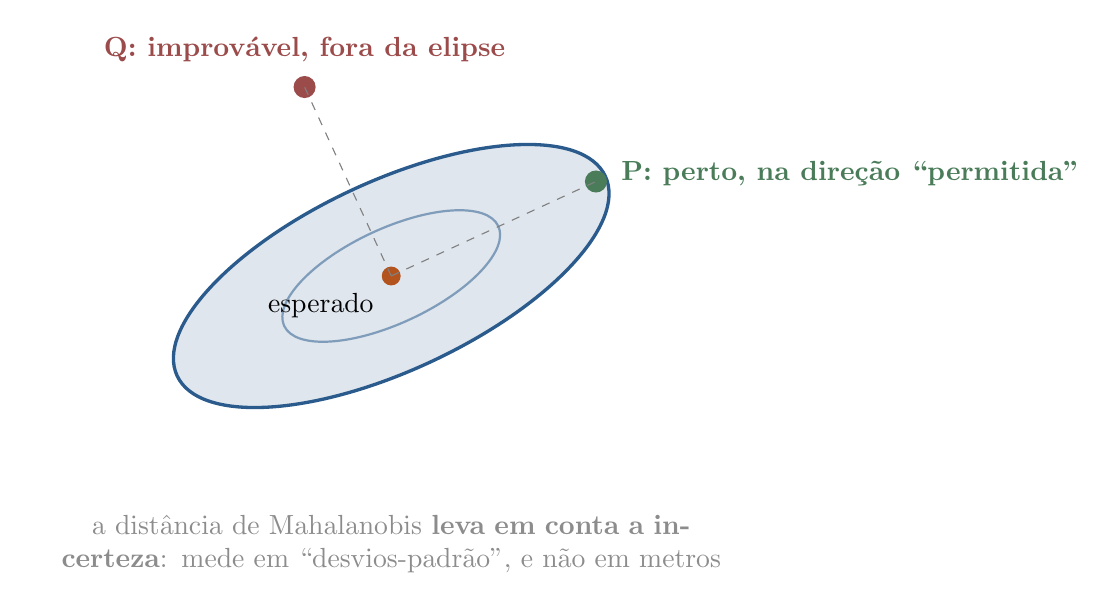
\begin{tikzpicture}[x=1cm,y=1cm,bal/.style={rectangle callout, rounded corners=7pt, draw=black!75, fill=white, line width=1pt, align=center, font=\normalsize, inner sep=5pt}]
\begin{scope}[rotate=25] \draw[dblue, fill=dblue!15, line width=1.2pt] (0,0) ellipse (3.0 and 1.2); \draw[dblue!60, line width=0.8pt] (0,0) ellipse (1.5 and 0.6); \end{scope}
\fill[dorange] (0,0) circle (0.12); \node[font=\normalsize, anchor=north east] at (-0.1,-0.1) {esperado};
\fill[dgreen] (2.6,1.2) circle (0.14); \node[dgreen, font=\normalsize\bfseries, anchor=west] at (2.8,1.3) {P: perto, na direção ``permitida''};
\fill[dred] (-1.1,2.4) circle (0.14); \node[dred, font=\normalsize\bfseries, anchor=south] at (-1.1,2.6) {Q: improvável, fora da elipse};
\draw[black!50, dashed] (0,0) -- (2.6,1.2); \draw[black!50, dashed] (0,0) -- (-1.1,2.4);
\node[dsub, font=\normalsize, align=center, text width=9cm] at (0,-3.4) {a distância de Mahalanobis \textbf{leva em conta a incerteza}: mede em ``desvios-padrão'', e não em metros};
\end{tikzpicture}
\end{document}
